\documentclass{scrartcl}

\usepackage[utf8]{inputenc}
\usepackage[T1]{fontenc}
\usepackage{lmodern}
\usepackage[ngerman]{babel}
\usepackage{amsmath}

\usepackage{hyperref}

\usepackage[justification=RaggedRight, singlelinecheck=false]{caption}
\usepackage{subcaption} 

\usepackage{listings}
\usepackage[usenames,dvipsnames]{xcolor}

% This is the color used for MATLAB comments below
\definecolor{MyDarkGreen}{rgb}{0.0,0.4,0.0}

% For faster processing, load Matlab syntax for listings

\lstloadlanguages{Matlab}%

\lstset{language=Matlab,                        % Use MATLAB
        frame=single,                           % Single frame around code
        basicstyle=\small\ttfamily,             % Use small true type font
        keywordstyle=[1]\color{Blue}\bfseries,        % MATLAB functions bold and blue
        keywordstyle=[2]\color{Purple},         % MATLAB function arguments purple
        keywordstyle=[3]\color{Blue}\underbar,  % User functions underlined and blue
        identifierstyle=,                       % Nothing special about identifiers
                                                % Comments small dark green courier
        commentstyle=\usefont{T1}{pcr}{m}{sl}\color{MyDarkGreen}\small,
        stringstyle=\color{Purple},             % Strings are purple
        showstringspaces=false,                 % Don't put marks in string spaces
        tabsize=5,                              % 5 spaces per tab
        %
        %%% Put standard MATLAB functions not included in the default
        %%% language here
        morekeywords={xlim,ylim,var,alpha,factorial,poissrnd,normpdf,normcdf},
        %
        %%% Put MATLAB function parameters here
        morekeywords=[2]{on, off, interp},
        %
        %%% Put user defined functions here
        morekeywords=[3]{FindESS, homework_example},
        %
        morecomment=[l][\color{Blue}]{...}    % Line continuation (...) like blue comment
}

% Includes a MATLAB script.
% The first parameter is the label, which also is the name of the script
%   without the .m.
% The second parameter is the optional caption.
\newcommand{\matlabscript}[2]
  {\begin{itemize}\item[]\lstinputlisting[caption=#2,label=#1]{#1.m}\end{itemize}}

\usepackage[edges]{forest}
\usetikzlibrary{shadows}
\definecolor{folderbg}{RGB}{124,166,198}
\definecolor{folderborder}{RGB}{110,144,169}

\newlength\Size
\setlength\Size{4pt}
\tikzset{%
  folder/.pic={%
    \filldraw [draw=folderborder, top color=folderbg!50, bottom color=folderbg] (-1.05*\Size,0.2\Size+5pt) rectangle ++(.75*\Size,-0.2\Size-5pt);
    \filldraw [draw=folderborder, top color=folderbg!50, bottom color=folderbg] (-1.15*\Size,-\Size) rectangle (1.15*\Size,\Size);
  },
  file/.pic={%
    \filldraw [draw=folderborder, top color=folderbg!5, bottom color=folderbg!10] (-\Size,.4*\Size+5pt) coordinate (a) |- (\Size,-1.2*\Size) coordinate (b) -- ++(0,1.6*\Size) coordinate (c) -- ++(-5pt,5pt) coordinate (d) -- cycle (d) |- (c) ;
  },
}

\forestset{%
  declare autowrapped toks={pic me}{},
  declare boolean register={pic root},
  pic root=0,
  pic dir tree/.style={%
    for tree={%
      folder,
      font=\ttfamily,
      grow'=0,
    },
    before typesetting nodes={%
      for tree={%
        edge label+/.option={pic me},
      },
      if pic root={
        tikz+={
          \pic at ([xshift=\Size].west) {folder};
        },
        align={l}
      }{},
    },
  },
  pic me set/.code n args=2{%
    \forestset{%
      #1/.style={%
        inner xsep=2\Size,
        pic me={pic {#2}},
      }
    }
  },
  pic me set={directory}{folder},
  pic me set={file}{file},
}

\usepackage{graphicx,import}
\usepackage{transparent}
\usepackage{float}

\title{Quick start Guide}
\author{Benjamin Schnabel}
\date{\today}

\begin{document}

\maketitle
\tableofcontents

\section{Verzeichnisstruktur}

In Abbildung \ref{fig:verzeichnisstruktur} ist eine Übersicht über die Verzeichnisstruktur des Modells zur Simulation der thermischen Eigenschaften beim Selektiven Lasersintern dargestellt. Dabei sind nur die wichtigsten Dateien aufgeführt und kurz erklärt.

\begin{figure}
\begin{forest}
pic dir tree,
pic root,
for tree={
	directory,
},
[\textbackslash
[{\hyperref[sec:laserModel]{Laser model}}
[{\hyperref[subsec:getLaserParameter]{getLaserParameter.m}}, file]
]
[Latex]
[{\hyperref[sec:materialModel]{Material model}}]
[{\hyperref[sec:reports]{Reports}}]
[{\hyperref[sec:stlFile]{STL file}}]
[{\hyperref[sec:thermalModel]{Thermal model}}
[{\hyperref[subsec:getThermalParameter]{getThermalParameter.m}}, file]
]
[{\hyperref[sec:usefulFunctions]{Useful functions}}
[{\hyperref[subsec:plotSimulation]{plotSimulation.m}}, file]
]
[{\hyperref[sec:main]{main.m}}, file]
]
\end{forest}
\caption{Verzeichnisstruktur}
\label{fig:verzeichnisstruktur}
\end{figure}

\section{Schnellstart}\label{sec:schnellstart}

Für den Schnellstart der Simulation wird die STL-Datei im Ordner \textit{STL file} abgelegt. Im Anschluss wird die Matlab-Datei \textit{main.m} geöffnet. In Abbildung \ref{fig:1} ist der Auswahldialog der STL-Datei dargestellt. In diesem wird einfach die zuvor abgelegte Datei ausgewählt. Im nächsten Schritt werden noch die wichtigsten Simulationsparameter abgefragt. Dies ist in Abbildung \ref{fig:2} dargestellt.

\begin{figure}
\centering
\begin{subfigure}[t]{0.4\textwidth}
\centering
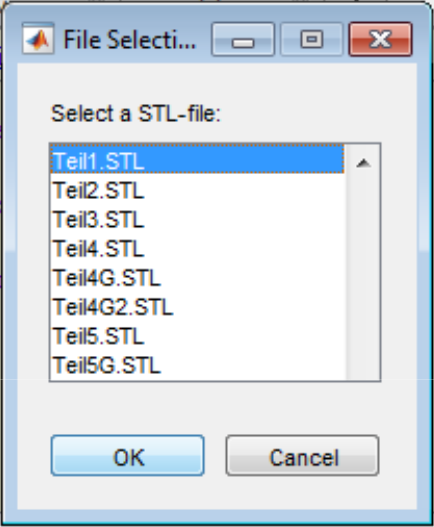
\includegraphics[width=\textwidth]{bild2.png}
\caption{STL-Datei Auswahldialog}
\label{fig:1}
\end{subfigure}
\begin{subfigure}[t]{0.55\textwidth}
\centering
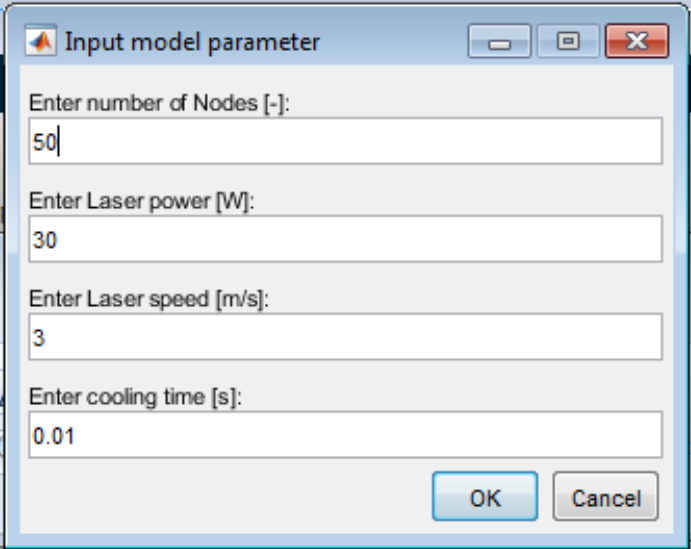
\includegraphics[width=\textwidth]{bild1.png}
\caption{Parametereingabe}
\label{fig:2}
\end{subfigure}
\caption{Blabka}
\end{figure}

\section{Laser model}\label{sec:laserModel}

Definition der Laserparameter.

\subsection{getLaserParameter}\label{subsec:getLaserParameter}

Hier werden die Laserleistung und die Scangeschwindigkeit festgelegt.

\begin{lstlisting}
function parameter = getLaserParameter()
    % Stefan-Boltzmann constant [W/(m^2 K^4)]
    parameter.stefanBoltzmanConstant = 5.670367 * 10^-8;
    % Focal length [mm]
    parameter.focalLength = 120.0;
    % Wave length [ym]
    parameter.waveLength = 10.63;
    % Laser power [W]
    parameter.laserPower = 30.0;
    % Raw beam radius at focusing lens [mm] 
    parameter.rawBeamRadius = 16.0;
    % Distance to focal point [mm]
    parameter.distanceFocalPoint  = 10.0;
    % Laser Speed [m/s]
    parameter.laserSpeed = 3.0;
end
\end{lstlisting}

\section{Material model}\label{sec:materialModel}

Definition der Werkstoffparameter.

\section{Reports}\label{sec:reports}

Nach jeder Simulation werden die erstellten Berichte in diesem Ordner automatisch abgelegt.

\section{STL file}\label{sec:stlFile}

Die erstellen STL-Dateien werden hier abgelegt.

\section{Thermal model}\label{sec:thermalModel}

Definition der thermischen Parameter.

\subsection{getThermalParameter}\label{subsec:getThermalParameter}

\begin{lstlisting}
function parameter = getThermalParameter()
    % Number of nodes
    parameter.numberOfNodes = 50;
    % Chamber temperature [K]
    parameter.chamberTemperature = 273.15 + 175.0;
    % Powderbed temperature [K]
    parameter.powderbedTemperature = 273.15 + 163.0;
    
    % Boltzmann constant [J/K]
    parameter.boltzmannConstant = 1.3806504 * 10^-23;
    % Speed of light [m/s]
    parameter.speedOfLight = 299792458;
    % Planck constant [Js]
    parameter.planckConstant = 6.62606896 * 10^-34;
    
    % Cooling time [s]
    parameter.coolingtime = 0.01;
end
\end{lstlisting}

\section{Useful functions}\label{sec:usefulFunctions}

\subsection{plotSimulation}\label{subsec:plotSimulation}

\section{main}\label{sec:main}

\begin{lstlisting}
stlName = 'Teil2.STL';
rotateZAxis = '0';
\end{lstlisting}

\section{Ablauf Simulation}

\begin{figure}
\centering
\def\svgwidth{350pt}
\input{Programmablaufplan.pdf_tex}
\caption{Programmablaufplan zur Durchführung der Simulation}
\label{fig:softwareablauf}
\end{figure}

\end{document}